
\chapter{Introduction}

This paper will begin by 

\section{Space of course explorers and schedulers}

%%%

\section{Overview of CDCS}

\label{fig:cdcs-index}

\subsection{``Better CDCS''}

\begin{figure}[ht]
    \centering
    \fbox{
        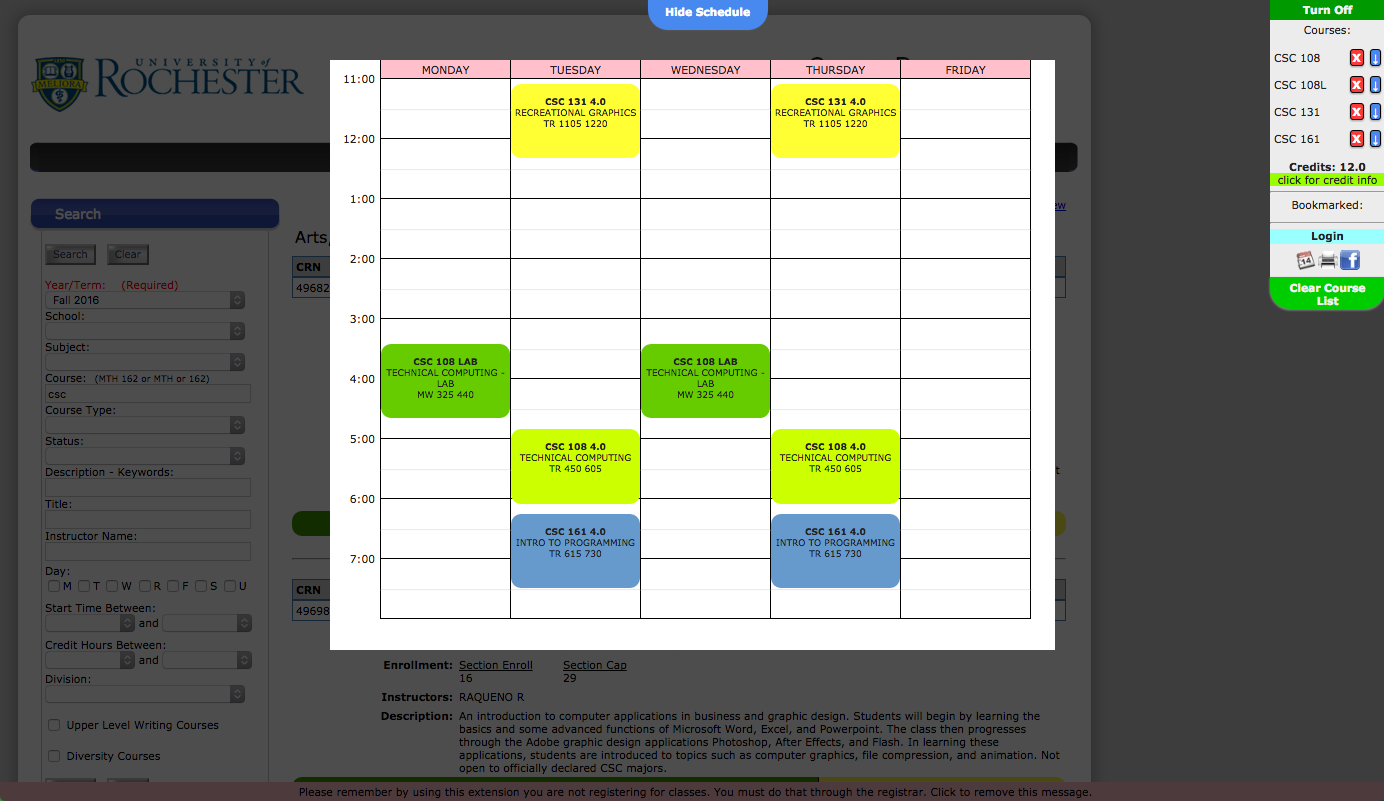
\includegraphics[width=1.00\textwidth]{images/cdcs/better}
    }
    \caption{Better CDCS, a separate browser extension that embeds buttons into the CDCS course results interface, allowing users to add courses to a locally-stored schedule}
    \label{fig:cdcs-better}
\end{figure}

%%%

\section{Overview of Skedge}

Skedge is a website I developed in 2014 and have been maintaining and developing since.

Bookmarks

Students, parents, department coordinators, and faculty can all benefit from such tool improvements.

\ref{fig:sk-index}


\begin{figure}[ht]
    \centering
        \begin{subfigure}[h]{14cm}
            \centering
            \fbox{
                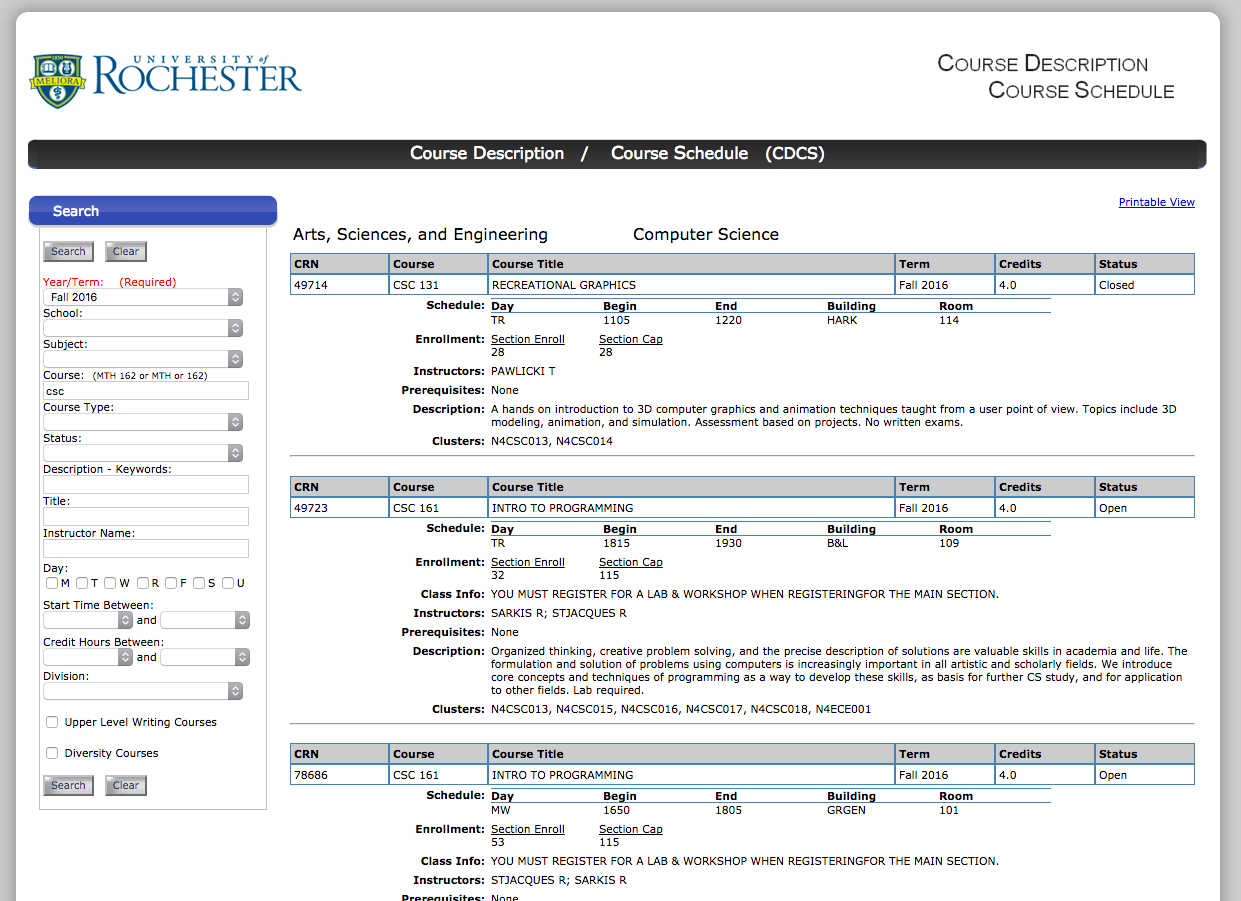
\includegraphics[width=1.00\textwidth]{images/cdcs/index}
            }
            \caption{CDCS}
            \label{fig:cdcs-index}
        \end{subfigure}\\
        \vspace{10pt}\\
        \begin{subfigure}[h]{14cm}
            \centering
            \fbox{
                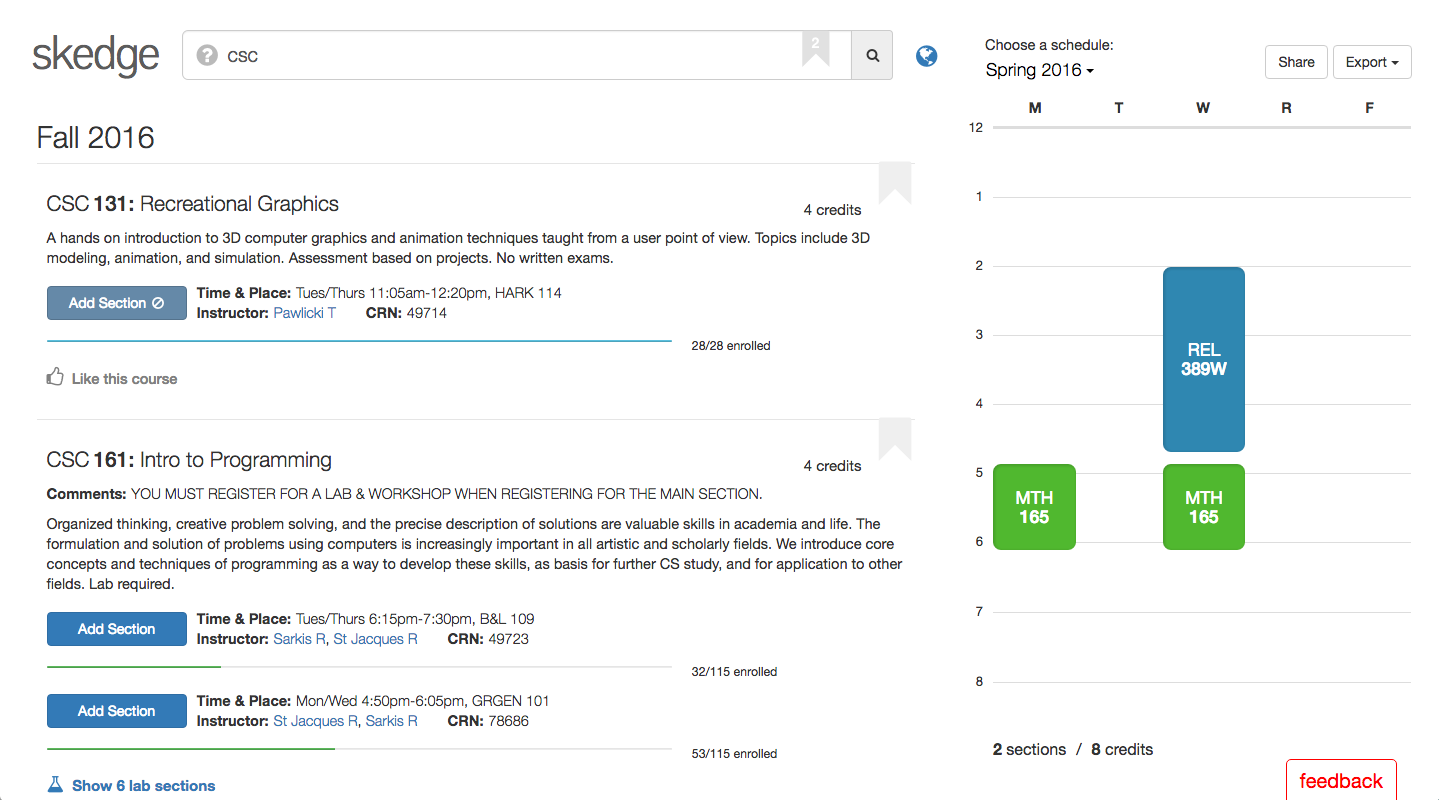
\includegraphics[width=1.00\textwidth]{images/skedge/index}
            }
            \caption{Skedge}
            \label{fig:sk-index}
        \end{subfigure}\\
        \vspace{20pt}\\
    \caption{CDCS and Skedge for the search query {\tt csc}}
\end{figure}

